% Asset ID: FA21ConicSections2EnrichmentTikZ-003
% Source: hyperbola sketching example
% Boundary status: Off-spec enrichment until official CCEA conics evidence is supplied.
\documentclass[tikz,border=8pt]{standalone}
\usepackage{amsmath,amssymb}
\usetikzlibrary{arrows.meta,calc,positioning}
\definecolor{Canvas}{HTML}{FAF9F6}
\definecolor{Ink}{HTML}{2C2C2E}
\definecolor{Gold}{HTML}{C5A059}
\definecolor{GoldDeep}{HTML}{D4AF37}
\begin{document}
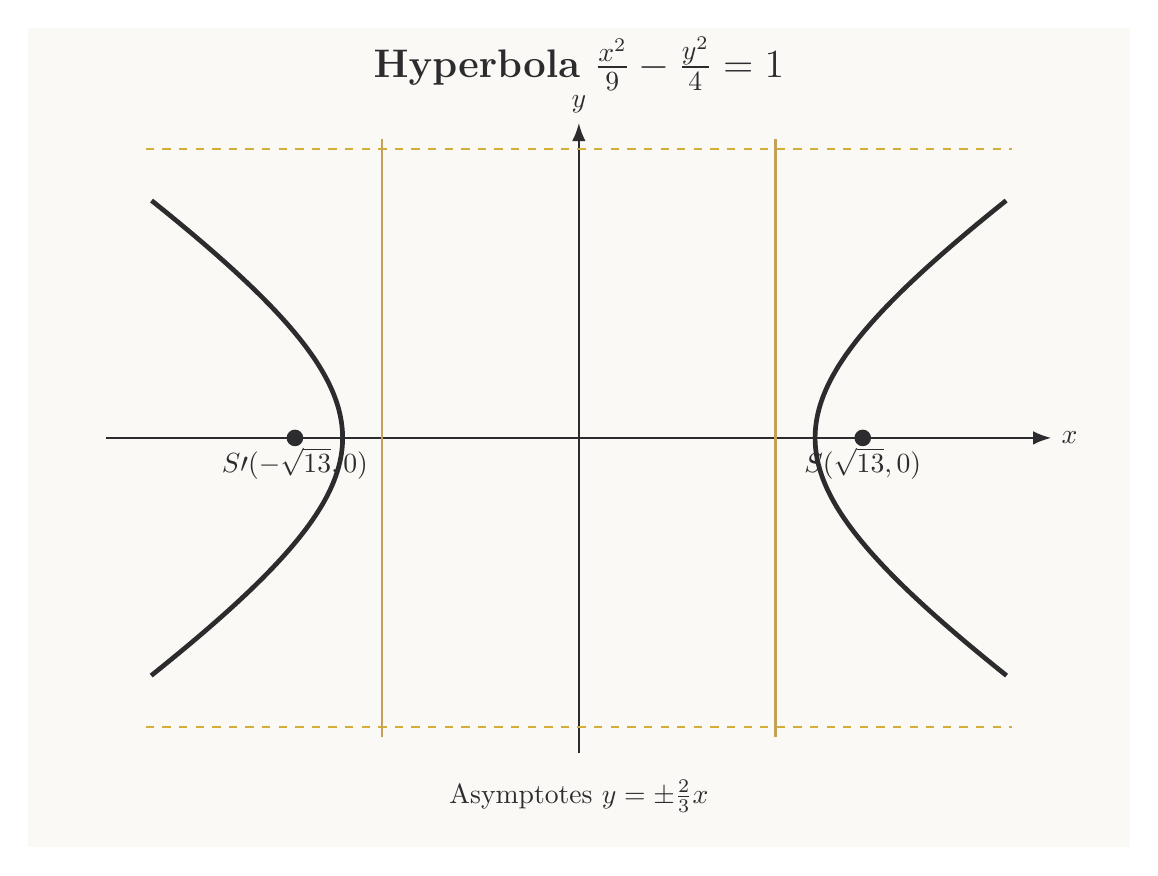
\begin{tikzpicture}[x=1cm,y=1cm,>=Latex]
\fill[Canvas] (-7,-5.2) rectangle (7,5.2);
\node[Ink, font=\Large\bfseries] at (0,4.75) {Hyperbola $\frac{x^2}{9}-\frac{y^2}{4}=1$};
\draw[Ink, thick, -Latex] (-6,0)--(6,0) node[right] {$x$};\draw[Ink, thick, -Latex] (0,-4)--(0,4) node[above] {$y$};\draw[GoldDeep, dashed, thick] (-5.5,{-2/3*(-5.5)})--(5.5,{2/3*5.5});\draw[GoldDeep, dashed, thick] (-5.5,{2/3*(-5.5)})--(5.5,{-2/3*5.5});\draw[Gold, thick] ({9/sqrt(13)},-3.8)--({9/sqrt(13)},3.8);\draw[Gold, thick] ({-9/sqrt(13)},-3.8)--({-9/sqrt(13)},3.8);\draw[Ink, line width=1.7pt, smooth, samples=140, domain=-1.2:1.2, variable=\t] plot ({3*cosh(\t)}, {2*sinh(\t)});\draw[Ink, line width=1.7pt, smooth, samples=140, domain=-1.2:1.2, variable=\t] plot ({-3*cosh(\t)}, {2*sinh(\t)});\fill[Ink] ({sqrt(13)},0) circle (3pt) node[below] {$S(\sqrt{13},0)$};\fill[Ink] ({-sqrt(13)},0) circle (3pt) node[below] {$S\prime(-\sqrt{13},0)$};\node[Ink] at (0,-4.55) {Asymptotes $y=\pm\frac23x$};
\end{tikzpicture}
\end{document}
